\documentclass{book}

\usepackage[utf8]{inputenc}
\usepackage{titlesec}
\usepackage{easylist}
\usepackage{hanging}
\usepackage{hyperref}
\usepackage[a4paper,top=2.0cm,bottom=2.0cm,left=2.0cm,right=3.0cm]{geometry}
\usepackage{blindtext}
\usepackage{tipa}
\usepackage{epigraph}
\usepackage{enumerate}
\usepackage{longtable}
\usepackage{setspace}
\usepackage{verbatim}
\usepackage[T1]{fontenc}
\usepackage{graphicx}
\usepackage[italian]{babel}
\usepackage{amsmath}
\usepackage{pbox}
\usepackage{fancyhdr}
\usepackage{cancel}
\usepackage{tabularx}
\usepackage{booktabs}
\usepackage{multirow}
\usepackage{longtable}
\usepackage{upgreek}
\usepackage{tikz}
\usepackage{tikz-qtree}
\usepackage{subfig}
\usepackage{xcolor}
\usepackage{amssymb}
\usepackage{mathrsfs}
\usepackage{textcomp}
\usepackage{circuitikz}
\usepackage{pifont}
\usepackage{mathtools}
\usepackage{amsmath}
\usepackage{listings}
\usepackage{color}
\usepackage{tasks}
\usepackage{amsthm}

\usetikzlibrary{angles, arrows.meta, quotes}
\usepackage{siunitx}

\definecolor{mygreen}{rgb}{0,0.6,0}
\definecolor{mygray}{rgb}{0.5,0.5,0.5}
\definecolor{mymauve}{rgb}{0.58,0,0.82}

\lstset{ 
  backgroundcolor=\color{white},   % choose the background color; you must add \usepackage{color} or \usepackage{xcolor}; should come as last argument
  basicstyle=\footnotesize,        % the size of the fonts that are used for the code
  breakatwhitespace=false,         % sets if automatic breaks should only happen at whitespace
  breaklines=true,                 % sets automatic line breaking
  captionpos=b,                    % sets the caption-position to bottom
  commentstyle=\color{mygreen},    % comment style
  deletekeywords={...},            % if you want to delete keywords from the given language
  escapeinside={\%*}{*)},          % if you want to add LaTeX within your code
  extendedchars=true,              % lets you use non-ASCII characters; for 8-bits encodings only, does not work with UTF-8
  firstnumber=1000,                % start line enumeration with line 1000
  frame=single,	                   % adds a frame around the code
  keepspaces=true,                 % keeps spaces in text, useful for keeping indentation of code (possibly needs columns=flexible)
  keywordstyle=\color{blue},       % keyword style
  language=Octave,                 % the language of the code
  morekeywords={*,...},            % if you want to add more keywords to the set
  numbers=left,                    % where to put the line-numbers; possible values are (none, left, right)
  numbersep=5pt,                   % how far the line-numbers are from the code
  numberstyle=\tiny\color{mygray}, % the style that is used for the line-numbers
  rulecolor=\color{black},         % if not set, the frame-color may be changed on line-breaks within not-black text (e.g. comments (green here))
  showspaces=false,                % show spaces everywhere adding particular underscores; it overrides 'showstringspaces'
  showstringspaces=false,          % underline spaces within strings only
  showtabs=false,                  % show tabs within strings adding particular underscores
  stepnumber=2,                    % the step between two line-numbers. If it's 1, each line will be numbered
  stringstyle=\color{mymauve},     % string literal style
  tabsize=2,	                   % sets default tabsize to 2 spaces
  title=\lstname                   % show the filename of files included with \lstinputlisting; also try caption instead of title
}

\linespread{1.5} % l'interlinea

\frenchspacing

\newcommand{\abs}[1]{\lvert#1\rvert}

\usepackage{floatflt,epsfig}

\usepackage{multicol}
\newcommand\yellowbigsqcup[1][\displaystyle]{%
  \fboxrule0pt
  \ifx#1\textstyle\fboxsep-0.6pt\else\fboxsep-1.25pt\fi
  \mathrel{\fcolorbox{white}{yellow}{$#1\bigsqcup$}}}

\title{Appunti Fisica}
\author{Nicola Ferru}
\date{}
\begin{document}
\maketitle
\tableofcontents
\listoftables
\listoffigures
% pagine dedicate
\section{Premesse\dots}
In questo repository sono disponibili pure le dimostrazioni grafiche realizzate
con \textit{Geogebra} consiglio a tutti di dargli un occhiata e di stare
attenti perché possono essere presenti delle modifiche per migliorare il
contenuto degli stessi appunti, comunque solitamente vengono fatte revisioni
tre/quattro volte alla settimana perché sono in piena fase di sviluppo. Ricordo
a tutti che questo è un progetto volontario e che per questo motivo ci
potrebbero essere dei rallentamenti per cause di ordine superiore e quindi
potrebbero esserci meno modifiche del solito oppure potrebbero esserci degli
errori, chiedo la cortesia a voi lettori di contattarmi per apportare una
modifica.
\begin{center}
	Cordiali saluti
\end{center}


\section{Simboli}
\begin{multicols}{3}
	$\in$ Appartiene\\
	$\notin$ Non appartiene\\
	$\exists$ Esiste\\
	$\exists !$ Esiste unico\\
	$\subset$ Contenuto strettamente\\
	$\subseteq$ Contenuto\\
	$\supset$ Contenuto strettamente\\
	$\supseteq$ Contiene\\
	$\Rightarrow$ Implica\\
	$\Longleftrightarrow$ Se e solo se\\
	$\neq$ Diverso\\
	$\forall$ Per ogni\\
	$\ni :$ Tale che\\
	$\leq$ Minore o uguale\\
	$\geq$ Maggiore o uguale\\
	$\alpha$ alfa\\
	$\beta$ beta\\
	$\gamma$ gamma\\
	$\Gamma$ Gamma\\
	$\delta,\Delta$ delta\\
	$\epsilon$ epsilon\\
	$\sigma,\Sigma$ sigma\\
	$\rho$ rho
\end{multicols}

\part{fisica 1}
\chapter{Grandezze fisiche e unità di misura}
In fisica, una grandezza è la proprietà di un fenomeno, corpo o sostanza, che può essere espressa quantitativamente mediante un numero e un riferimento (ovvero che può essere misurata quantitativamente). by \href{https://it.wikipedia.org/wiki/Grandezza_fisica}{Wikipedia}
\begin{table}[!h]
	\centering
	\begin{tabular}{lll}
		\texttt{Grandezza}&\texttt{Nome}&\texttt{Simbolo}\\\hline
		Tempo&secondo&Simbolo\\
		Lunghezza&metro&m\\
		Quantità di materiale&mole&mol\\
		Temperatura termodinamica&kelvin&K\\
		Corrente elettrica&ampere&A\\
		Intensità luminosa&candela&cd\\\hline
	\end{tabular}
\caption{Unità fondamentali del sistema internazionale}
\label{table:1}
\end{table}\\
Per una questione di comodità di lettura esistono i multipli delle unità di
misura e vengono indicati con dei prefissi che consente di risurre il numero di
cifre, rendere più veloce la lettura e la scrittura.
\begin{table}[!h]
	\centering
	\begin{tabular}{cll|cll}
		\texttt{Fattore}&\texttt{Prefisso}&\texttt{Simbolo}&\texttt{Fattore}&\texttt{Prefisso}&\texttt{Simbolo}\\\hline
		$10^{18}$&exa-&E&$10^{-1}$&deci-&d\\
		$10^{15}$&peta-&P&$10^{-2}$&centi-&c\\
		$10^{12}$&tera-&T&$10^{-3}$&milli-&m\\
		$10^{9}$&giga-&G&$10^{-6}$&micro-&$\mu$\\
		$10^{6}$&mega-&M&$10^{-9}$&nano-&$n$\\
		$10^{3}$&kilo-&k&$10^{-12}$&pico-&$p$\\
		$10^{2}$&etto-&h&$10^{-15}$&femto-&$f$\\
		$10^{1}$&deca-&da&$10^{-18}$&atto-&$a$\\\hline

	\end{tabular}
\caption{Prefissi per le unità SI$^a$}
\end{table}
\section{Sistema internazionale delle unità di misura}
l sistema internazionale di unità di misura (in francese: \textit{Système international d'unités}), abbreviato in S.I. (pronunciato esse-i
), è il più diffuso sistema di unità di misura. Nei paesi anglosassoni sono ancora impiegate delle unità consuetudinarie, un esempio sono quelle statunitensi.
La difficoltà culturale nel passaggio della popolazione da un sistema all'altro è essenzialmente legato a radici storiche. Il sistema internazionale impiega per la maggior parte unità del sistema metrico decimale nate nel contesto della rivoluzione francese: le unità S.I. hanno gli stessi nomi e praticamente la stessa grandezza pratica delle unità metriche. Il sistema è un sistema tempo-lunghezza massa che è stato inizialmente chiamato Sistema MKS, per distinguerlo dal similare Sistema CGS. Le sue unità di misura erano infatti metro, chilogrammo e secondo invece che centimetro, grammo, secondo. By \href{https://it.wikipedia.org/wiki/Sistema_internazionale_di_unità_di_misura}{Wikipedia}

\chapter{I moti}
\section{Moto uniforme rettilineo}
\begin{equation}
	x=v*t+x_0
\end{equation}
Un punto \textit{P} si muove sull'asse \textit{y} con $v=4\frac{m}{s}$ e
posizione iniziale $-6m$. Determina la legge del moto. Dopo quanto tempo
$y=24m$. Quel è lo spazio percorso dopo 8 secondi.
\begin{equation}
	\begin{matrix}
		y=v*t+y_0\\
		\boxed{y=4*t-6}\\
	\end{matrix}
\end{equation}
Il passaggio successivo è quello di ricavare il tempo, per fare questo
operazione sarà necessario fare i seguenti passaggi
\begin{equation}
	\begin{matrix}
		y=4*t-6\\
		y+6=4t \text{ porto } y_0 \text{ al primo termine}\\
		t=\frac{y+6}{4}=\frac{24+6}{4}=\frac{30}{4}=7,5s\\
		t=0\to y_0=-6m\\
		t=8\to y=4*8-6=26m\\
		\Delta y=y-y_0=26-(-6)=32m
	\end{matrix}
\end{equation}
Quindi alla fine lo spazio percorso è di 32m.
\section{moto rettilineo uniformemente accelerato}
Moto rettilineo uniformemente accelerato. La definizione di moto rettilineo
uniformemente accelerato è: il moto di un corpo con accelerazione costante
lungo una traiettoria retta sempre nella stessa direzione e identico verso. Le
formule utilizzate in questo tipo di esercizio sono sostanzialmente due:
\begin{equation}
	\begin{matrix}
			v=a*t+v_0&\text{retta}\\
			y=\frac{1}{2}*t^2+v_0*t+y_0&\text{parabola}
	\end{matrix}
\end{equation}
\subsection{Un esempio}
Un punto P si muove con $a=2m/s^2$, $v_0=5m/s$, $y_0=-60m$\\
Scrivi: le leggi del moto, la velocità e la distanza dell'origine dopo 8
secondi.
\subsubsection{soluzione}
\begin{multicols}{2}
	\begin{equation}
	\begin{matrix}
			v=a*t+v_0\\
			v=2*t+5\\
	\end{matrix}
	\end{equation}
	\begin{equation}
	\begin{matrix}
			y=\frac{1}{2}*t^2+v_0*t+y_0\\
			y=\frac{1}{2}*2^2+5*t-60\\
			y=t^2+5t-60
	\end{matrix}
	\end{equation}
	Per verificare che quello che abbiamo ottenuto sia quanto meno giusto
	dobbiamo in primo luogo constatare che $v=y^\prime$ quindi se il valore
	della derivata prima di $y$ sarà uguale a $v$ vuol dire che le formule
	ottenute sono giuste.
\end{multicols}
\paragraph{Verifica} \[v=\frac{dy}{dt}=y^\prime=2t+5\] Questa è la prova che il
lavoro svolto ha dato i dovuti risultati.\\
Adesso la prima cosa da fare è proprio quella di sostituire $t$ con il proprio
valore.
\begin{equation}
	\begin{matrix}
			t=8s&\to&v=2*8+5=21m/s\\
			t=8s&\to&y=(8)^2+5(8)-60\\
			&&y=64+40-60\\
			&&y=44m
	\end{matrix}
\end{equation}
Una domanda comunque potrebbe essere la seguente: ``\textit{Qual'è lo spazio
percorso dal 5° al 9° secondo?}''. Sostanzialmente andremo a studiare lo
spostamento in quel lasso di tempo. Di sicuro bisogna calcolare lo spostamento
nei due punti, prendendoli singolarmente in un primo momento, quindi
\begin{equation}
	\begin{matrix}
		t_1=5s&\to&y_1=(5)^2+5(5)-60=25+25-60=10m\\
		t_2=9s&\to&y_2=(9)^2+5*(9)-60=81-45-60=-24m
	\end{matrix}
\end{equation}
Ovviamente adesso manca lo spazio percorso, per ottenere questo valore sarà
necessario calcolare il discriminante, il suddetto $\Delta y$.
\begin{equation}
	\boxed{
		\begin{matrix}
			\Delta y=y_2-y_1\\
			\Delta y=-24-(-10)=-24+10=-14m
		\end{matrix}
	}
\end{equation}
Quindi la distanza percorsa in quel lasso di tempo è 14 metri in negativo.
\subsection{Un problema tipico}
Un punto A si muove con $a=-1,5m/s^2$, $v_0=70m/s$, $y_0=-300m$. Scrivi le leggi
del moto. Dopo quanto tempo la velocità è 25 m/s? In tale tempo che spazio
percorre?
\subsubsection{Soluzione}
Il primo punto è quella di ricavare le formule sostituendo i valori che
conosciamo.
\begin{equation}
	\begin{matrix}
		v=at+v_0&y=\frac{1}{2}at^2+v_0t+y_0\\
		v=1,5t+70&y=\frac{1}{2}(1,2)t^2+70+300\\
		&y=-0,75t^2+70t-300
	\end{matrix}
\end{equation}
il secondo punto è quello di ricavare il tempo impiegato
\begin{equation}
	\begin{matrix}
		t=0&\to&y_0=-300m\\
		t=30&\to&y=-0,75*(30)^2+70*30-300=-675+2100-300=1125m
	\end{matrix}
\end{equation}
Dopo aver svolto questi due passaggi, possiamo iniziare a a calcolare i punti i
punti necessari a calcolare la distanza percorsa.
\begin{equation}
	\begin{matrix}
		\Delta y=y-y_0\\
		\Delta y=1125-(-300)=1425m
	\end{matrix}
\end{equation}

\subsection{Esercitazione 1}
Si lascia cadere un sasso in un pozzo. Se il tonfo nell'acqua viene percepito
con un ritardo di 2,40s a quale distanza dell'imboccatura del pozzo si trova la
superficie del l'acqua? La velocità del suono nell'aria è 336m/s. E se non teniamo conto del tempo cui il suono impiaga ad arrivare fino a noi, che errore percentuale commettiamo? Nel calcolare la profondità a cui si trova acqua?
\begin{equation*}
	V_{s}=336m/s\text{ } \Delta t_{tot}=2,40s \text{ legge oraria del sasso che cade}
\end{equation*}
\begin{multicols}{2}
	\begin{equation*}
		y(t)=y_0+V_0t+\frac{1}{2}at^2
	\end{equation*}
	\begin{equation*}
		y(t)=h-\frac{1}{2}gt^2
	\end{equation*}
	\begin{equation*}
		y_0=h
	\end{equation*}
	\begin{equation*}
		V_0=0
	\end{equation*}
	\begin{equation*}
		a=-g=9,81m/s^2
	\end{equation*}
\end{multicols}
\begin{equation*}
	\Delta t=t_{caduta}-t_{suono}
\end{equation*}
\begin{multicols}{2}
	\begin{equation*}
		h=V_0t_{suono}
	\end{equation*}
	\begin{equation*}
		t_{suono}=\frac{h}{V_s}
	\end{equation*}
	\begin{equation*}
		\begin{cases}
			y(t_{(caduta)}=0)=0 \\
			h-\frac{1}{2}gtc^2=0
		\end{cases}
	\end{equation*}
	\begin{equation*}
		tc=\sqrt{\frac{2h}{g}}
	\end{equation*}
\end{multicols}
\begin{equation*}
	\Delta t_{tot}=\sqrt{2h}{g}+\frac{h}{V_0}\to \frac{\sqrt{2h}}{g}=\Delta t_{tot} - \frac{h}{V_s}\to \frac{2h}{g}\to \frac{2h}{g}=\bigg(\Delta t-\frac{h}{V_s}\bigg)^2
\end{equation*}
\begin{equation*}
	\Rightarrow (\Delta t)^2+\frac{h^2}{V_{s^2}} -\frac{2h}{V_s}\Delta t=\frac{2h}{g}\to (\Delta t)^2-2 \bigg(\frac{\Delta t}{V_s}+\frac{1}{g}\bigg) h+\frac{h^2}{V_{s^2}} =0 
\end{equation*}
\paragraph{Forma ridotta\label{forma ridotta es.1.1}}
\begin{equation*}
	h^2-V_{s^2}\bigg(\frac{\Delta t+st}{V_s}+\frac{1}{g}\bigg)h+V_{s^2}\Delta t_{tot}^2=0
\end{equation*}
\begin{equation*}
	h=V_{s^2}\bigg(\frac{\Delta t_{tot}}{V_0}+\frac{1}{g}\bigg)\pm \sqrt{V_{s^2}\bigg(\frac{\Delta}{V_s}+\frac{1}{g}\bigg)^2-V^2_s\Delta t^2_{tot}}
\end{equation*}
\begin{equation*}
	h=V_{s^2}\bigg(\frac{\Delta t_{tot}}{V_s}+\frac{1}{g}\bigg)-\sqrt{V_{s^2}\bigg(\frac{\Delta t}{V_s}+\frac{1}{g}\bigg)^2-V_{s^2}\Delta t^2}\Rightarrow \Delta t_{tot}-\frac{h}{V_s}>0
\end{equation*}
\subsection{Esercitazione 2}
In un particolare gioco per bambini una pallina di massa 50.0 grammi viene lanciata su una pista orizzontale   che   in   un   certo   punto   inizia   a   piegarsi   per   formare   un   anello   verticale   completo  e circolare di raggio $R= 51.0 cm$.  Per lanciare la pallina si usa una molla di costante elastica $kel=100N/m$. Di quanto deve essere compressa la molla per poter fornire alla pallina la velocità  minima chele permette di non cadere nel punto più alto (\textit{si trascurino le forze di attrito; PRECISAZIONE: LA MASSA SCIVOLA SENZA ATTRITO}). 
\subsubsection{Soluzione}
Si può applicare il teorema di conservazione dell’energia meccanica considerando, per l’istante $t_1$, l’energia potenziale elastica associata alla massa ferma sulla molla compressa e per l’istante  $t_2$, l’energia  meccanica  della  massa  nel  punto  più  alto  ($2=h_R$)  della  sua  traiettoria.  Precisamente, possiamo scrivere:
\begin{equation*}
	K_1+U_1=K_2+U_2
\end{equation*}
Dove  $K_1$  e  $K_2$  sono le energie cinetiche negli istanti  $t_1$  e  $t_2$, rispettivamente, e  $U_1$  e  $U_2$  sono le energie potenziali negli istanti $t_1$ e $t_2$, rispettivamente. Sulla base delle indicazioni fornite dal testo del problema, possiamo scrivere
\begin{equation*}
	\begin{matrix}
		K_1=0;&K_2=\frac{1}{2}mv_2^2;&U_2=\frac{1}{2}k\Delta x_m^2;&U_2=mgh=2mgR
	\end{matrix}
\end{equation*}
dove $k$ è la costante elastica della molla, $\Delta x_m$ è la deformazione in compressione della molla, $v_2$ è la velocità della massa nel punto più alto della traiettoria. Al riguardo, la forza vincolare, ossia quella che costringe la massa a seguire la traiettoria circolare, può considerarsi nulla nel momento in cui si studia il problema nella condizione limite di ``distacco'' dalla pista. Ne segue che la sola forza che agisce sulla massa e, in modulo, $mg$. Dunque, essendo g perpendicolare alla velocità, risulta essere, all’istante $t_2$ anche l’accelerazione normale, ossia
\begin{equation*}
	a=g \to \frac{v_2^2}{R}=g\to v_2^2=gR\to K_2=\frac{1}{2}mbR
\end{equation*}
Pertanto, facendo le opportune sostituzioni, si ottiene
\begin{equation*}
	\frac{1}{2}k\Delta x_n^2=\frac{1}{2}mv_2^2\to \frac{1}{2}\Delta x_m^2=\frac{5}{2}mgR\to|\Delta x_mg|=\sqrt{\frac{5mgR}{k}}
\end{equation*}
\subsection{Esercitazione 3}
Una turbina idraulica è azionata da una corrente d'acqua ad alta velocità che urta contro le pale e rimbalza.   In   condizioni   ideali,   la   velocità   delle   particelle   d'acqua   dopo   l'urto   contro   la   pala   è esattamente nulla così che tutta l'energia dell'acqua si è trasferita alla turbina. Se la velocità delle particelle dell'acqua è 27.0 m/s, quanto vale la velocità ideale della pala della turbina? (\textit{Si consideri l'urto di una particella d'acqua contro la pala come un urto unidimensionale elastico})
\subsubsection{Soluzione}
La massa della singola molecola d’acqua è estremamente piccola rispetto a quella della pala, cosìche si può trattare il problema come quello dell’urto elastico unidimensionale di una massa m suuna parete (massa virtualmente infinita). Sappiamo che nelle suddette condizioni, nel sistema diriferimento in cui la parete e ferma, il modulo della velocità della massa rimane la stessa prima edopo l’urto. Precisamente, posto $v^\prime_1>0$  la proiezione sull’asse x (direzione dell’urto) del vettore velocità all’istante  $t_1$  (poco prima dell’urto), nel sistema di riferimento in cui la parete è ferma, e $v^\prime_2>0$  la proiezione sull’asse x del vettore velocità all’istante $t_1$ (poco dopo l'urto), nello stesso sistema di riferimento, risulta
\begin{equation*}
	v^\prime_2=v^\prime_1
\end{equation*}
Il testo del problema ci fornisce i dati delle velocità ($v_1=27.0m/2$ $v_2=0$) nel sistema di riferimento di terra, quello in cui la pala (parete) si muove con velocità incognita V (la pala si muove a regime costante e non cambia la sua velocità). Usando le relazioni di trasformazione delle velocità  tra sistemi di riferimento in moto relativo con velocità V possiamo scrivere
\begin{eqnarray*}
	v_1=V+v^\prime_1\\
	v_2=V+v^\prime_2
\end{eqnarray*}
sommando membro a membro e tenendo conto che $v_2=0$ si ottiene 
\begin{equation*}
	v_1=2V\to V=v_1/2
\end{equation*}
\subsection{Esercitazione 4}
Un pacco è lasciato cadere su un nastro trasportatore orizzontale. La massa del pacco è m, la velocità del nastro trasportatore è v e il coefficiente di attrito dinamico per il pacco sul nastro è $\mu d$. Per quanto tempo il pacco striscerà sul nastro? Qual è la distanza percorsa dal pacco durante l'intervallo di tempo calcolato nel punto precedente?
\subsubsection{Soluzione}
La forza di attrito si oppone allo scivolamento del pacco e, pertanto, trascina il pacco accelerandolo nel verso del moto del nastro. La forza di attrito è anche la risultante delle forze che agiscono sul pacco. Precisamente,
\begin{eqnarray*}
	m\overrightarrow{a}=\overrightarrow{F}_r=\overrightarrow{F}_{att}\\
	||\overrightarrow{F}_{att}||=\mu_dmg;&F_{att,x};&ma_x=\mu_dmg
\end{eqnarray*}
dove si è  preso come asse x quello corrispondente alla direzione del nastro, e come verso positivo quello corrispondente al moto del nastro, che è anche il verso del vettore accelerazione. Il pacco striscerà fino a quando raggiungerà la stessa velocità del nastro (il moto relativo diventa nullo). Pertanto, l’intervallo di tempo richiesto risulta
\begin{equation*}
	v=a:x\Delta t=\mu_dg\Delta t\to \Delta t=\frac{v}{\mu_dg}
\end{equation*}
La distanza percorsa si ricava usando le note relazioni della cinematica del moto con accelerazione costante
\begin{equation*}
	\Delta x=\frac{1}{2}\frac{v^2}{\mu_dg}
\end{equation*}
Si può risolvere il problema seguendo altri percorsi, tutti molto semplici. Ad esempio, si può studiare il problema nel sistema di riferimento del nastro. Supponiamo allora che il nastro si muova nel senso delle x negative. Rispetto al nastro (fermo) il pacco si muoverà con una velocità iniziale $v$ nel senso delle x positive. La forza di attrito, questa volta, ha componente negativa perché tendea frenare il moto del pacco rispetto al nastro ecc. ecc.
\subsection{Esercitazione 5}
Due vettori a e b hanno modulo uguale di 12,7 unità. Sono orientati come in
figura e la loro somma vettoriale è r. Trovare:
\begin{tasks}
	\task le componenti $x$ e $y$ di \textbf{r}
	\task il modulo di r;
	\task l'angolo che \textbf{r} forma con l'asse \textit{x}.
\end{tasks}
\begin{figure}[!ht]
	\centering
	\begin{tikzpicture}
		\node[] (pic) at (0,0) {\includegraphics[height=4cm]{img/esercizio 5
		im1.pdf}};
	\end{tikzpicture}
	\caption{figura 1}
\end{figure}
\begin{multicols}{2}
	Con questa formula ricavo il vettore \textbf{r}
	\begin{equation*}
		|\overrightarrow{a}|=|\overrightarrow{b}|=12.7
	\end{equation*}
	\begin{equation*}
		\alpha=28.2^o
	\end{equation*}
	\begin{equation*}
		\beta=115^o
	\end{equation*}
	\begin{equation*}
		\overrightarrow{r}=(r_x,r_y)=r_x \hat{i}+r_y*\hat{i}=(a_x+b_x, a_y+b_y)
	\end{equation*}
	\begin{equation*}
		\overrightarrow{r}=\overrightarrow{a}+\overrightarrow{b}
	\end{equation*}
\end{multicols}
\begin{multicols}{2}
	\begin{equation*}
		a_x=|\bar{a}|\cos \alpha=12.7\cos 28.2^o=11.2
	\end{equation*}
	\begin{equation*}
		a_y=|\bar{a}|\sin \alpha=12.7\sin 28.2^o=6
	\end{equation*}
	\begin{equation*}
		\sigma=180^o-\alpha-\beta=46,8^o
	\end{equation*}
	\begin{equation*}
		b_x=-|\overrightarrow{b}|\cos \sigma=-8.7
	\end{equation*}
	\begin{equation*}
		b_y=|\overrightarrow{b}|\sin \sigma=9.3
	\end{equation*}
\end{multicols}
	\begin{equation*}
		\overrightarrow{r}=(11.2-8.7,6+9.3)=(2.5,15.3)
	\end{equation*}
	\begin{equation*}
		|\overrightarrow{r}|=\sqrt{r^2_x+r^2_y}=\sqrt{2.5^2+15.3^2}=15.5
	\end{equation*}
	\begin{equation*}
		r_x=|\overrightarrow{r}|*\cos \delta
	\end{equation*}
	\begin{equation*}
		r_x=|\overrightarrow{r}|*\cos \delta
	\end{equation*}
	\begin{equation*}
		\cos \delta=\frac{r_x}{|\overrightarrow{r}|}
	\end{equation*}
	\begin{equation*}
		\delta=\arccos\left(\frac{r_x}{\abs{\overrightarrow{r}}}\right)=80.7^o
	\end{equation*}
	\begin{equation*}
		V_1=100km/h=\frac{100}{3.6}\frac{m}{s}=27.9m/s
	\end{equation*}
	\begin{equation*}
		V_2=130km/h=36.1m/s
	\end{equation*}
	\begin{equation*}
		\Delta t=3.0min=180s
	\end{equation*}
\subsection{Esercitazione 6}
	\begin{equation*}
		V_1=100km/h=\frac{100}{3.6}\frac{m}{3.6}\frac{m}{s}=27.8m/s
	\end{equation*}
	\begin{equation*}
		V_2=100km/h=130km/h=36*1m/s
	\end{equation*}
	\begin{equation*}
		\Delta t=3.0min=180s
	\end{equation*}
	\begin{equation*}
		S(t)=S_0+vt
	\end{equation*}
	\begin{equation*}
		\text{camion: } s_1(t)=S_0+r_1t \text{ } s_0=v_1*\Delta
		t=27.8m/s*180s=5*10^3m
	\end{equation*}
	\begin{equation*}
		\text{auto: } s_2(t)=v_2*t
	\end{equation*}
	\begin{equation*}
		s_1(t_f)=s_2(t_f)
	\end{equation*}
\begin{multicols}{2}
	\begin{equation*}
		s_0+r_1t_f=v_2f_y
	\end{equation*}
	\begin{equation*}
		s_1=v_2t_f-v_1t_f=t_f(v_2-v_1)
	\end{equation*}
	\begin{equation*}
		\boxed{t_f=\frac{s_0}{v_2-v_1}}=\frac{5*10^3m}{(36.1-27.8)m/s}=602s=10min
	\end{equation*}
	\begin{equation*}
		s_1(t_f)=s_0+v_1t_f=5*10^3m+27.8m/s*602s=21735m=22km
	\end{equation*}

\end{multicols}
\subsection{Esercitazione}
Un punto P si muove di MUD con $a=-0,8m/s^2$, $v_0=90m/s$, $y_0=-60m$. Scrivi
la legge del moto. Dopo quanto tempo la velocità è 25m/s. Quel è lo spazio
percorso dal 3° secondo al 7° secondo.
\subsubsection{Soluzione}
Il primo passo è quello di calcolare le due formule necessarie per svolgere
questo esercizio, quindi ci ricaviamo le due leggi del moto uniformemente
accelerato.
\begin{equation*}
	\begin{matrix}
		v=at+v_0&y=\frac{1}{2}at^2+v_0t+y_0\\
		v=-0,8t+90&y=\frac{1}{2}\left(-0,8\right)t^2+90t-60
	\end{matrix}
\end{equation*}
Dopo averle ricavate possiamo ottenere il tempo dalla formula della velocità
\begin{equation*}
	t=\frac{-v+90}{0,8}=\frac{-25+90}{0,8}\simeq81,2s
\end{equation*}
Ovviamente, adesso bisogna ricavare il percorso, quindi andiamo a sostituire
\begin{equation*}
	\begin{matrix}
		t=0&\to&y_0=-60m\\
		t=81,2&\to&\frac{1}{2}\left(-0,8\right)(81.2)^2+90*81-60\simeq 4611
	\end{matrix}
\end{equation*}
Ora dobbiamo calcolare il discriminante per calcolare quanto ha percorso in
81,2 secondi.
\begin{equation*}
	\begin{matrix}
		\Delta y=y-y_0\\
		\Delta y=4611-(-60)=4611+60=4671m
	\end{matrix}
\end{equation*}
Quindi il nostro punto P ha percorso circa 4671 metri in totale.
Visto che l'esercizio chiede di calcolare il percorso effettuato dal 3° secondo
al settimo dobbiamo ripetere la sostituzione effettuata prima per stimare il
percorso completo, sostituendo i due t con i secondi in questione.
\begin{equation*}
	\begin{matrix}
		t=3&\to&\frac{1}{2}\left(-0,8\right)(3)^2+90*3-60=206,4\\
		t=7&\to&\frac{1}{2}\left(-0,8\right)(7)^2+90*7-60=550,4
	\end{matrix}
\end{equation*}
E poi ricalcoliamo il discriminante
\begin{equation*}
	\begin{matrix}
		\Delta y=y-y_0\\
		\Delta y=550,4-206,4=344m
	\end{matrix}
\end{equation*}
Quindi da questo si può dedurre che il percorso in quel lasso di tempo è di 344
metri.

\chapter{Modelli atomici}
\section{Modello atomico di Bohr-Sommerfeld}
Il modello atomico proposto da Niels Bohr nel 1913, successivamente ampliato da Arnold Sommerfeld nel 1916, è la più famosa applicazione della quantizzazione dell'energia che, insieme alle spiegazioni teoriche sulla radiazione del corpo nero, sull'effetto fotoelettrico e sullo scattering Compton, e all'equazione di Schrödinger, costituiscono la base della meccanica quantistica.\\
Il modello, proposto inizialmente per l'atomo di idrogeno, riusciva anche a spiegare, entro il margine di errore statistico, l'esistenza dello spettro sperimentale. Bohr presenta così un modello dell'atomo, facendo intuire che gli elettroni si muovono su degli orbitali. \textit{Questo modello viene ancora utilizzato nello studio dei Semiconduttori.} 
\begin{center}
	By \href{https://it.wikipedia.org/wiki/Modello_atomico_di_Bohr}{Wikipedia}
\end{center}
\part {Fisica 2}
\chapter{programma}
\section{Base}
\begin{itemize}
	\item \textit{Elettrostatica nel vuoto} - carica elettrica, legge di Coulomb, campo elettrico, teorema di Gauss e $1^a$ equazione di Maxwell, potenziale elettrico, dipolo elettrico, conduttori, capacità elettrica, sistemi di condensatori, collegamento in serie e in parallelo, energia del campo elettrostatico.
	\item \textit{Corrente elettrica stazionaria} - resistenza elettrica e legge di Ohm, effetto Joule, forza elettromotrice e generatori elettrici, circuiti in corrente continua.
	\item \textit{Magnetismo nel vuoto} - forza di Lorentz, vettore induzione magnetica, forze magnetica
	 su una corrente, momento magnetico della spira percorsa da corrente, relazione tra momento
	 meccanico e momento magnetico, campi generati da correnti stazionarie, legge di Biot e Savart (campo
	 del filo indefinito, della spira circolare e del solenoide), 2a equazione di Maxwell, teorema di Ampère.
	\item \textit{Campi magnetici variabili nel tempo} - induzione elettromagnetica , legge di 
	Faraday-Newmann, $3^a$ e $4^a$ equazione di Maxwell, autoinduzione, circuito RL, 
	energia magnetica.
	\item \textit{Onde} - equazione d'onda, tipi di onde, velocità di fase, equazioni delle onde
	elettromagnetiche e loro proprietà, onda piana e onde sferiche, energia di un'onda 
	elettromagnetica e vettore di Poynting, spettro della radiazione elettromagnetica. 
\end{itemize}
\section{Argomenti aggiuntivi}
\begin{itemize}
	\item \textit{Elettrostatica nella materia} - la costante dielettrica, interpretazione microscopica, suscettibilità elettrica.
	\item \textit{Magnetismo nella materia} - vettori B, H e M, materiali paramagnetici, ferromagnetici, diamagnetici, legge di Curie, ciclo di isteresi.
\end{itemize}

\chapter{La legge di Couloumb}
\section{Introduzione}
L'elettromagnetismo costituisce il fondamento su cui sono costruiti i computer,
le radio e televisori, le telecomunicazioni, illuminazioni ecc.
L'elettromagnetismo spiega come gli atomi siano tenuti insieme, come
avvengono i fulmini, le aurore e gli arcobaleni. Gli antichi filosofi greci
scoprirono che l'ambra strofinata attrae pagliuzze sottili e che pietre
magnetiche naturali attraggono pezzetti di ferro. Tra i tanti scienziati che
svilupparono l'elettromagnetismo moderno, notiamo il fisico sperimentale
\texttt{Michael Faraday} ed il teorico \texttt{James Clerk Maxwell}.
\subsection{La carica elettrica}
Una bacchetta di vetro strofinata con seta si \texttt{allontana} da un'altra
bacchetta di vetro strofinata con della seta.
\begin{enumerate}
	\item \textit{Forza repulsiva} - Una bacchetta di vetro strofinata con
		della seta si \textit{avvicina} ad una bacchetta di plastica strofinata
		con la pelle di camoscio.
	\item \textit{Forza attrattiva} - Le forze sono dovute alla \textbf{carica
		elettrica}.
\end{enumerate}
Esistono due tipi di carica:
\begin{enumerate}
	\item Carica positiva, contrassegnata con il segno +;
	\item Carica negativa, contrassegnata con il segno -
\end{enumerate}
Si definisce neutro un oggetto che ha le cariche positive e negative
perfettamente bilanciate.
Spostando la carica da un oggetto all'altro, si crea una carica in eccesso.
L'oggetto può scaricarsi con scintille oppure con l'umidità dell'aria.
\subsubsection{Le proprietà delle cariche}
\begin{enumerate}
	\item Le particelle cariche dello \textit{stesso segno} si respingono;
	\item Le particelle di carica opposta si attraggono;
	\item Se strofiniamo il vetro con un panno di seta risulta in una
		\textit{carica potenziale} nel vetro;
	\item Strofinando della plastica con della pelle di camoscio si ottiene una
		\textit{carica negativa} sulla stessa.
\end{enumerate}
\subsubsection{Conduttori e isolanti}
In natura esistono le seguenti tipologie di materiali:
\begin{tasks}{2}
	\task I conduttori - le cariche si muovono liberamente;
	\task Gli isolanti - le cariche non si muovono, per l'appunto restano
	isolate;
	\task I semiconduttori - le cariche si muovono, ma il materiale possiede un
	alta resistenza;
	\task I superconduttori - le cariche si muovono senza incontrare ostacoli
	di sorta.
\end{tasks}
\newtheorem{pcariche}{Particelle Cariche}
\begin{pcariche}
	La materia composte di atomi. Gli atomi hanno un \textbf{nucleo} con
	\begin{itemize}
		\item Protoni - cariche positive;
		\item Elettroni - carica negativa.
	\end{itemize}
	La carica dell'elettrone e del protone hanno la stessa intensità ma segno
	opposto. Gli elettroni sono \textbf{attratti verso il nucleo}. Nei
	conduttori, alcuni elettroni sono \textit{liberi di muoversi}, un isolante
	\textit{non ha elettroni liberi}.
\end{pcariche}
\subsection{Carica indotta}
Una carica negativa \textit{respinge} gli elettroni nel rame, risulta una
carica positiva indotta vicino alla carica esterna. Risulta una \textbf{forza
attrattiva} tra una carica negativa e un conduttore, Anche per una carica
positiva ed un conduttore la forza risulta \textbf{attrattiva}.
\section{Legge di Coulomb}
Tra due cariche puntiformi esiste una \textit{forza elettrostatica}. La forza è
diretta \textit{lungo la retta congiungente} le due cariche.
Se le cariche sono della stessa polarità le stesse si respingono, invece, se
sono di carica opposta, avviene un attrazione tra le cariche.
\subsubsection{Riassunto sui vettori}
\paragraph{Componenti:}
\begin{equation}
	F_x=F\cos 0;\text{ }F_y=F\sin 0
\end{equation}
\paragraph{Modulo e angolo:}
\begin{equation}
	F=\abs{\vec{F}}=\sqrt{F_x^2+F_y^2};\text{ } \tan 0 =\frac{F_y}{F_x}
\end{equation}
\paragraph{Versore:}
\begin{equation}
	\hat{a}=\frac{\vec{a}}{\abs{\vec{a}}}=\frac{\vec{a}}{a}
\end{equation}
\paragraph{Sommare:}
\begin{equation}
	\vec{F}=\vec{F}_1+\vec{F}_2\to F_x=F_{1x}+F_{2x};\text{ } F_y=F_{1y}+F_{2y}
\end{equation}
La forza di una carica $q_1$ in presenza di un'altra $q_2$ è:
\begin{equation}
	\vec{F}_{12}=k\frac{q_1q_2}{r^2}\hat{r}
\end{equation}
Dove $k=8,99*10^9Nm^2C^{-2}$ è la \textbf{costante di Coulomb} e $\vec{r}$ è il
vettore di lunghezza pare alla distanzia $q_2$ a $q_1$.
\begin{enumerate}
	\item Se $q_1$ e $q_2$ hanno la stessa polarità, il prodotto $q_1q_2$ è 
		\textbf{positivo} e la forza è \textit{repulsiva}.
	\item Se $q_1$ e $q_2$ hanno la polarità \textbf{opposta}, il
		prodotto $q_1q_2$ è \textbf{negativo} e la forza è \textit{attrattiva}.
\end{enumerate}
La forma è una coppia di azione-reazione: $\vec{F}_{21}=-\vec{F}_{12}$
\subsection{Unità do misura}
L'unità di carica nel SI è il \texttt{Coulomb} (\ref{}). La derivata del unità
fondamentale di corrente elettrica, \textbf{Ampere}. La corrente \textit{i} è
data dal rapporto $\frac{dq}{dt}$ con cui transita la carica \textit{q}: 
$i=\frac{dq}{dt}$.
Risulta $1C=1As$
\subsection{La costante dielettrica del vuoto}
La costante di \textit{Coulomb} viene anche espressa come
$k=\frac{1}{4\pi\xi_0}$ dove $\xi_0 = 8,85*10^{-12}C^2N^{-1}m^{-2}$ è la
\textbf{constante dielettrica del vuoto}.\\
Così scriviamo $\vec{F}=\frac{q_1q_2}{4\pi\xi_0r^2}\hat{r}$, o per ottenere il
modulo $F=\frac{\abs{q_1}\abs{q_2}}{4\pi\xi_0r^2}\hat{r}$
\subsection{Forze multiple}
Le forze elettrostatiche obbediscono al \textbf{principio di sovrapposizione}.
Se molte particelle sono vicine alla carica $q_1$, la forza netta è $\vec{F}_{1,net}=\vec{F}_{12}+\vec{F}_{14}+\dots+\vec{F}_{1n}$.
\paragraph{Attenzione:} \textit{somma vettoriale!}
\section{Teorema del guscio}
\begin{tasks}(2)
  \task Primo teorema del guscio:\\
  \textit{Una superficie sferica uniformemente carica attrae o respinge una carica esterna come se tutta la carico fasse concentroto
    nel suo centro}.
  \task Secondo teorema del guscio:\\
  \textit{Uno carico posto all'interno di uno superficie chiusa uniformemente carica non ne sente la foza}.
\end{tasks}
\section{La quantizzazione della carica}
Qualunque carica \textit{q} può essere scritta come $q=ne$ in cui $n=\pm 1,\pm 2, \pm 3, \dots$ ed è la carica elementare: $e = 1,602*10^{-19}C$
\begin{tasks}
  \task Il \textbf{protone} ha carica $+e$
  \task L'ettrone ha carica $-e$
\end{tasks}

Il valore di e è così piccolo che normalmente la granularità non appare nei fenomeni di larga scala. Attraverso un filo con corrente di 1A passano circa $6,2*10^{18}$ elettroni al secondo.

\section{La conservazione della carica}
La carica elettrica è conservata - Lo strofinamento del vetro con un panno di seta non crea carica positiva, ma trasferisce elettroni dal vetro alla seta. Anche nei processi nucleari la carica totale rimane invariata.
\section{Verifica}
\begin{enumerate}
\item Indicare il verso della forza che agisce sul protone centrale
\item Ordinare i tre casi secondo i valori decrescenti del modulo della forza netta sull'elettrone.
\end{enumerate}
\paragraph{Soluzione primo problema}
\begin{equation}
  q_1=+e,q_2=+2e, \text{ } R=2cm.
\end{equation}
Calcolo la forza $\vec{F}_{12}$
\begin{equation}
  F_{12}=k\frac{\abs{q_1}\abs{q_2}}{R^2}=k\frac{2e^2}{R^2}=\frac{8,99*10^9*2*(1,6*10^{19})}{R^2}=1,15*10^{-24}N
\end{equation}
Quindi il valore finale è $\vec{F}_{12}=-(1,15*10^{-24}N)\hat{x}$
\begin{equation}
  q_1=+e, q_2 = +2e,q_3=-2e, R=2cm.
\end{equation}
Calcolo la forza $\vec{F}_{1,net}$
\begin{equation}
 F_{13}=k\frac{2e^2}{\left(\frac{3}{4}R\right)^2}=2,05*10^{-24}N
\end{equation}
Quindi il valore che otteniamo è $F_{13}=(2,05*10^{-24}N)$
\begin{equation}
  \begin{matrix}
  \vec{F}_{1,net}=\vec{F}_{12}+\vec{F}_{13}=-(1,15*10^{-24}N)\hat{x}+(2,05*10^{-24}N)
    \hat{x}\\=(0,90*10^{24}N)\hat{y}=-(0,125*10^{-24}N)\hat{x}+(1,775*10^{-24}N)\hat{y}
  \end{matrix}
\end{equation}
Quindi il valore che otteniamo è $F_{1,net,x}=\sqrt{F^2_{1,net,x}+F^2_{1,net,y}}=1,78*10^{-24}N$
\paragraph{Soluzione secondo problema}
$q_1=8e,\text{ } q_2=-2e$. In che punto un protone è in equilibrio?
\begin{equation}
  \begin{matrix}
    \vec{F}_1+\vec{F}_2=0. \text{ } x>L.\text{ } \frac{kq_1e}{x^2}+\frac{kq_2e}{(x-L)^2}=0\\
    \to \left(\frac{x-L}{x}\right)=\frac{-q_2}{q_1}=\frac{1}{4}\to \frac{x-L}{x}=\frac{1}{2}\to x=2L
  \end{matrix}
\end{equation}


\chapter{Campi elettrici}
\section {L'aspetto fisico}
La forza elettrostatica tra 2 cariche sembra una ``azione a distanza''
\begin{itemize}
\item Spiegazione alternativa:\\
  \textit{La carica 1 crea un campo elettrico nello spazio circostante}\\
  \textit{La carica 2 sente l'effetto del campo 1}\\
\item vice versa:\\
  \textit{La carica 2 crea un campo elettrico nello spazio circostante}\\
  \textit{La carica 1 sente l'effetti del campo 2}
\end{itemize}
\section {Il campo elettrico}
\begin{tasks}{2}
\task campo scalare: temperatura, pressione, densità
\task campo vetoriale: velocità, accelerazione, forza
\end{tasks}
La forza $\vec{F}$ su un \textbf{carica esplorativa} $q_0$ determina il campo elettrico $\vec{E}$:
\begin{equation}
  \vec{E}=\frac{\vec{F}}{q_0}
\end{equation}
$\vec{E}$ è un campo vettoriale. Nel SI ``Sistema Internazione'', si esprime in N/C (o V/m)
\section{Linee di campo elettrico}
Per visualizzare $\vec{E}$, disegnamo delle linee:
\begin{itemize}
	\item Il vettore $\vec{E}$ è \textbf{tangente} alla linea 
	\item La \textbf{densità} delle linee rappresenta $\abs{\vec{E}}$
        \item Le linee \textbf{escono} dalle cariche positive
        \item Le linee \textbf{entrano} nelle cariche negative
\end {itemize}
\section {Altro esempio delle linee di campo}
\begin{figure}[!h]
 	\centering
	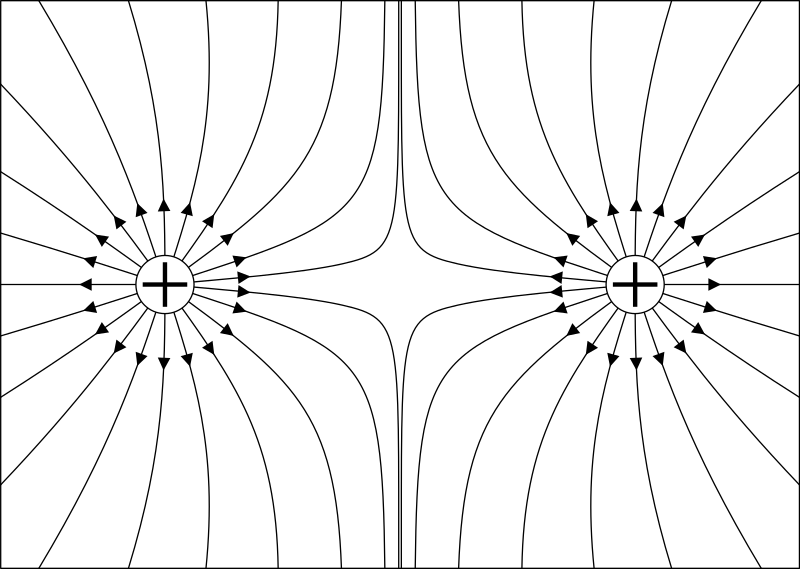
\includegraphics[height=4cm]{img/linee elettriche repulsione.png}
\end{figure}
Due cariche positive identifiche\\
Sempre:
\begin{itemize}
\item Il vettore $\vec{E}$ è tangente alla linea
\item La densità delle linee rappresenta $\abs {\vec{E}}$
\item Le linee escono dalla cariche positive
\item Le linee entrano nelle cariche negative
\end{itemize}
Il disegno stesso suggersce l'idea di una repulsione
\section{Campo $\vec{E}$ di una carica puntiforme}
Una carica esploratrice positiva $q_0$ attorno ad una \textit{carica puntiforme} $q$ sente una forza $\vec{F}=\frac{qq_0}{4\pi \xi_0r^2}\hat{r}$. \\
Per il campo $\vec{E}$ troviamo:
\begin{equation}
	\vec{E}=\frac{\vec{F}}{q_0}=\frac{q}{4\pi \xi_0r^2}\hat{r}
\end{equation}
La direzione di $\vec{E}$ è \textbf{radiale}
\begin{enumerate}
\item Per $q>0$, il verso di $\vec{E}$ è uscente
\item Per $q<0$, il verso di $\vec{E}$ è entrante
\end{enumerate}
Per il \textbf{modulo:} $E=\abs{\vec{E}}=\frac{\abs q}{4\pi \xi_0r^2}$  
\section{Il principio di sovrapposizione}
In presenza di \textbf{più cariche}, le forze obbediscono al principio di sovrapposizione:
\begin{equation}
  \vec{F}_0=\vec{F}_{01}+\vec{F}_{02}+\dots+\vec{F}_{0n}
\end{equation}
Il principio di sovrapposizione vale anche per $\vec{E}$:
\begin{equation}
  \vec{E}=\frac{\vec{F}_0}{q_0}+\frac{\vec{F}_{01}}{q_0}+\frac{\vec{F}_{02}}{q_0}+\dots+\frac{\vec{F}_{0n}}{q_0}=\vec{E}_1+\vec{E}_2+\dots+\vec{E}_n
\end{equation}
Il campo $\vec{E}$ di più particelle cariche è la somma vettoriale dei singoli contributi
\section{Verifica}
\begin{center}
\begin{tikzpicture} 
 \filldraw 
(0,0) circle (0pt) node[align=left,   below] {}      --
(1,0) circle (2pt) node[align=center, below] {S}     -- 
(4,0) circle (3pt) node[align=right, below] {e}     -- 
(5,0) circle (2pt) node[align=right,  below] {R}     --
(8,0) circle (3pt) node[align=right, below] {P}     --
(10,0) circle (0pt) node[align=left, below] {x};
\end{tikzpicture}
\end{center}
Il disegno mostra un elettrone ($e$) e un protone ($p$) sull'asse $x$
\begin{itemize}
	\item Indicare la direzione di \textit{E} dovuta all’elettrone nel
           punto \textit{S} e nel punto \textit{R}
        \item Indicare la direzione di \textit{E} dovuta al protone nel
punto \textit{S} e nel punto \textit{R}
\end{itemize}
\subsection {Soluzione}
\begin{equation}
  \begin{matrix}
    q_1=+2e\\
    q_2=-2e\\
    q_3=-4e
  \end{matrix}
\end{equation}
Ovviamente il primo passo da fare è quello di ricavare $\vec{E}$ nel origine
\begin{equation}
  E_1=E_2=\frac{2e}{4\pi\xi_0d^2}
\end{equation}
\begin{equation}
	E_3=\frac{4e}{4\pi\xi_0d^2}
\end{equation}
Ora ricaviamo $E_x$ tramite una somma tra $E_{1x}$, $E_{2x}$ e $E_{3x}$.
\begin{equation}
	E_x=E_{1x}+E_{2x}+E_{3x}=\frac{2e}{4\pi\xi_0d^2}\cos{30^o}+\frac{2e}{4\pi\xi_0d^2}\cos{30^o}+\frac{4e}{4\pi\xi_0d^2}\cos{30^o}=\frac{8e}{4\pi\xi_0d^2}\cos{30^o}
\end{equation}
\begin{equation}
	E_x=E_{1y}+E_{2y}+E_{3y}=\frac{-2e}{4\pi\xi_0d^2}\cos{30^o}+\frac{-2e}{4\pi\xi_0d^2}\cos{30^o}+\frac{4e}{4\pi\xi_0d^2}\cos{30^o}=0
\end{equation}
\section{Campo $\vec{E}$ di un dipolo elettrico}
Due particelle cariche, $-q$ e $+q$ separate da distanza $d$ e sull'asse dipolare $z$. Il prodotto $qd$ viene chiamato \textbf{momento di dipolo elettrico}: $p=qd$ e $\vec{p}$ vettoriale.
\begin{itemize}
\item direzione: l'asse dipolare
\item verso: da $-q$ a $+q$
\end{itemize}
Il campo $\vec{E}$ sull'asse dipolare distante $z$ dal centro del dipolo:
\begin{equation}
  \begin{matrix}
    E=E_+-E_-=\frac{q}{4\pi \xi\left(z-\frac{d}{2}\right)^2}-\frac{q}{4\pi \xi\left(z-\frac{d}{2}\right)^2}
    =\frac{q}{4\pi\xi_0}\frac{\left(z-\frac{d}{2}\right)^2-\left(z-\frac{d}{2}\right)^2}{\left(z-\frac{d}{2}\right)^2\left(z-\frac{d}{2}\right)^2}
    =\frac{q}{4\pi\xi_0}\frac{2zd}{\left(\left(z-\frac{d}{2}\right)^2\right)^{2}}\\
    =\frac{qd}{2\pi\xi_0z^3}\left(1-\left(\frac{d}{2z}\right)^2\right)^{-2}
    \end{matrix}
\end{equation}
Per $z>>d$ troviamo $E(z)=\frac{p}{2\pi\xi_0z^3}$, anche fuori dell'asse $z$, $E\propto r^{-3}$ per $r>>d$\\
Materiale isolandte (\textbf{e. g. plastica}). Raggio \textit{R}, carica \textbf{superficiale} $\sigma$ - Punto \textit{P} sull'asse centrale, direzione \textit{z}. Ogni anello ha carica $dq=\sigma 2\pi rdr$ e contribuisce a $dE=\frac{zdq}{4\pi\xi_0\left(4r^2+z^2\right)^{\frac{3}{2}}}$
\begin{equation}
  E=\inf dE=\int^R_0\frac{z\sigma2\pi rdr}{4\pi\xi_0\left(4r^2+z^2\right)^{\frac{3}{2}}}=\frac{z\sigma}{4\xi_0}\left[\frac{\left(4r^2+z^2\right)^{-\frac{1}{2}}}{-\frac{1}{2}}\right]^R_0
\end{equation}
Il risultato è $E=\frac{\sigma}{2\xi_0}\left(1-\frac{z}{\sqrt{R^2+z^2}}\right)$. Per $z<<R$ troviamo $E=\frac{\sigma}{2\xi_0}$.\\
Su una carica $q$ in un campo elettrico esterno $\vec{E}$ agisce un forza elettrostatica $\vec{F}=q\vec{E}$
\begin{itemize}
  \item per $q>0$, $\vec F$ ha lo stesso orientamento di $\vec E$
  \item per $q<0$, $\vec F$ ha l'orientamento opposto di $\vec E$
\end{itemize}
NB: Una carica non sente il proprio campo elettrico esterno!
\section{Misura della carica elementare}
\subsection{Millikan 1910}
\fbox{
 	\addtolength{\linewidth}{-2\fboxsep}%
 	\addtolength{\linewidth}{-2\fboxrule}%
	\begin{minipage}{\linewidth}
          L'esperimento di Millikan per antonomasia è l'esperimento della goccia d'olio, il cui obiettivo, cioè
          misurare la carica elettrica dell'elettrone, fu raggiunto nel 1909. Il valore ricavato da Robert
          Millikan fu $4,774(5) x 10^{-10}$ statcoulomb, equivalenti a $1,5924(17)x10^{-19}$ coulomb, minore
          dello 0,6\% circa rispetto a quello oggi comunemente accettato, pari a $1,602176634 x 10^{-19}$ coulomb.
        \end{minipage}
}
\begin{center}
  \href{https://it.wikipedia.org/wiki/Esperimento_di_Millikan}{By Wikipedia}
\end{center}
\subsubsection{Problema svolto}
Una goccia con $m=1,3*10^{-10}$, $Q=-1,5*10^{-13}C$ e $V_x=18m/s$ attraverso una zona di lunghezza $L=1,6cm$ e campo elettrico $E=1,4*10^6N/C$ verso il basso,
Qual'è la deflessione verticale?
\begin{equation}
  y=\frac{1}{2}at^2=\frac{1}{2}\frac{EQ}{m}\left(\frac{L}{vx}\right)^2=6,4*10^{-4}m=0,64mm
\end{equation}
\section{Prodotto scalare}
Esistono due prodotti tra vettori: il \underline{prodotto calare} e il \underline{prodotto vettoriale}.\\
Il prodotto scalare è appunto uno scalare (un \textbf{singolo numero}) funzione di due vettori, indicato con
$s=\vec{A}*\vec{B}$ e perciò anche detto \textbf{dot product}. Operativamente, posto $\abs{A}$ il modulo del vettore $\vec{A}$, $\abs{B}$ il modulo del vettore $\vec{B}$, e $\alpha$ l'\textbf{angolo} compreso tra i due vettori, il prodotto scalare si calcola con
\begin{equation}
	s=\vec{A}*\vec{B}=\abs{\vec{A}}\abs{\vec{B}}\cos \alpha
\end{equation}
Oppure equivalentemente, poste $A_x$ ecc. le componenti dei vettori comme la somma e i prodotti delle componenti
omologhe
\begin{equation}
  \vec{A}*\vec{B}=A_xB_x+A_yB_y+A_zB_z
\end{equation}
L'interpretazione geometrica è che il prodotto scalare è la \textbf{proiezione} di uno dei due vettori
sull'altro.
\section{Prodotto vettoriale}
Il prodotot vettoriale è un vettore funzione di due vettori, è si indica con $\vec{V}=\vec{A}*\vec{B}$ oppove
$\vec{V}=A\textturnv \vec{B}$. È anche detto \textbf{cross product}. Il modulo
$\abs{\vec{V}}=\vec{A}*\vec{B}\sin0$.\\
$\vec{V}$ è \textbf{perpendicolare} a $\vec{A}$ e a
$\vec{B}:\vec{V}\bot \abs{\vec{A}},\abs{\vec{V}}\bot\abs{\vec{B}}$. Il verso di $\vec{V}$ è determinato della
regola della mano destra: girando le dita da $abs{A} \text { a } \vec{B}$, il pollice indica il verso di $\vec{V}$. L'espressione esplicita è
\begin{equation}
  \vec{V}=(A_yB_z-A_zB_y)\hat{x}+(A_zB_x-A_xB_z)\hat{y}+(A_xB_y-A_yB_x)\hat{z}
\end{equation}
oppure si ottiene del \textbf{determinante:}
\begin{equation}
  \vec{V}=\begin{vmatrix}
            \hat{x}&\hat{y}&\hat{z}\\
            A_x&A_y&A_z\\
            B_x&B_y&B_x
          \end{vmatrix}
\end{equation}
\section{Dipolo in un campo elettrico}
In acqua ($H_2O$), il lato ossigeno è leggermente più negativo di quello dell'idrogeno. Posto in un campo
elettrico esterno $\vec{E}$, \textbf{si comporta come un dipolo} generico. Il \textbf{momento di dipolo elettrico} $\vec{p}$ è diretto lungo l'asse di simmetria della molecola e ha verso dalla carica negativa alla carica positiva.
\begin{equation}
  p(H_2O)=6,2*10^{-30}Cm
\end{equation}
Dipolo rapprensentato da due cariche $-q$ e $+q$ a distanza $d$. Il momento dipolo elettrico
$\vec{p}$ forma un angolo di $\texttheta$ col campo elettrico esterno $\vec{E}$ (uniforme)\\
\begin{figure}[!h]
 	\centering
	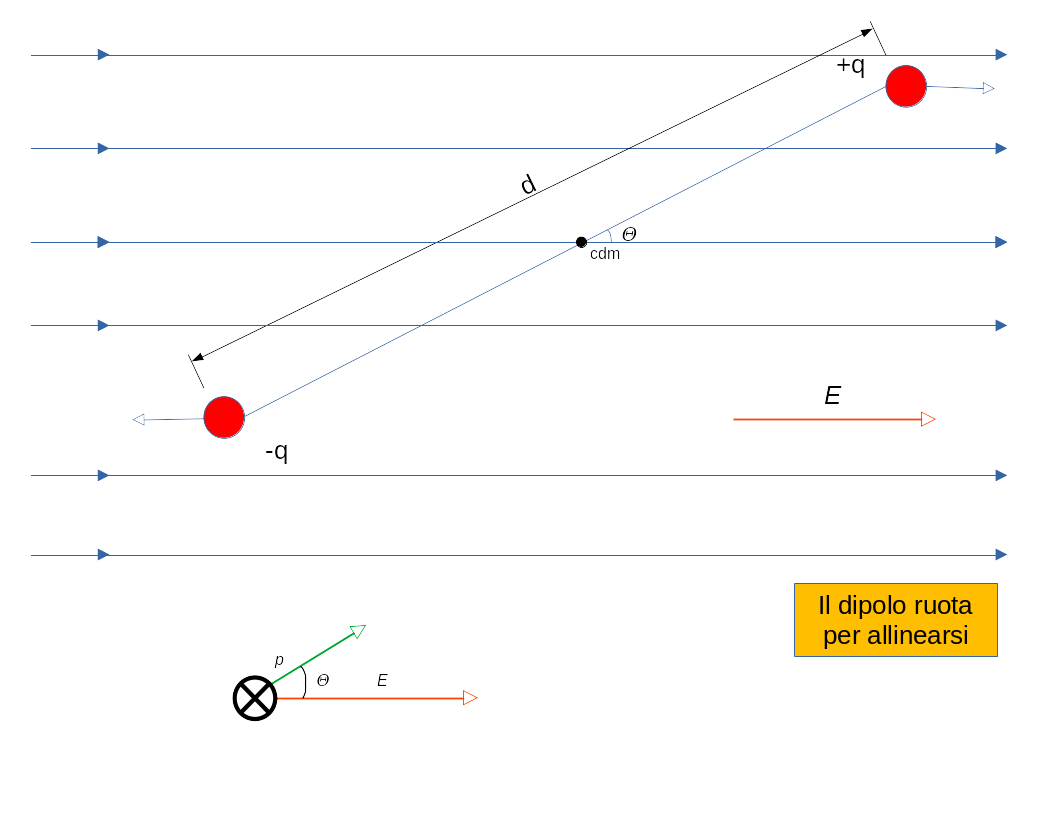
\includegraphics[height=8cm]{img/grafuci del dipolo elettrico.png}
\end{figure}
$\vec{F} (+q) e \vec{F} (-q)$ hanno intensità uguali e direzioni opposta. La forza netta è zero, ma esercitano un \textbf{momento torcente} $\vec{\uptau}$:
\begin{equation}
\uptau=-Fd \sin {\texttheta} = -pE sin {\texttheta}
\end{equation}
(\textit{segno meno perché il verso è orario}).
In forma vettore: $\vec{\uptau}=\vec{p}*\vec{E}$
\section{Energia potenziale di un dipolo elettrico}
L'energia potenziale $U$ di un dipolo elettrico $\vec{p}$ dipende dal suo \textit{orientamento}.
$U$ è minimo quando $\vec{p}$ è allineaTo Con il campo $\vec{E}$ - Nel mimimo è in equilibro:
$\abs{\vec{\uptau}}=\abs{p}\abs{E}\sin \texttheta=0$. Scegliamo $U=0$ per $\texttheta=90^o$.\\
L'energia potenziale diventa
\begin{equation}
  U=-L=\int^{\texttheta}_{90^o}\uptau d \texttheta= \int^{\texttheta}_{90^o} pE\sin \texttheta d\texttheta =-pE\cos\texttheta
\end{equation}
In forma vettoriale: $U=-\vec{p}*\vec{E}$
\section{Problema}
\begin{tasks}
  \task A quale distanza si trovano i cewntri delle cariche positiva e negativa di una molecola d'acqua?
  \begin{eqnarray*}
    p=qd\to d=\frac{p}{q}\\
    p(H_2O)=10e=1,6*10^{-30}C\\
    q(H_2O))10e)=1,6*10^{-18}C\\
    d=\frac{p}{q}=\frac{6,2*10^{-30}Cm}{1,6*10^{-18}C}=3,9*10^{-12}m=3,9pm
  \end{eqnarray*}
  \task Qual'è la differenza di energia potenziale tra le orientazioni $\texttheta=0^o$ e $\texttheta=180^o$ in un campo esterno $E=1,5*10^4\frac{N}{C}$?
  \begin{equation}
	\Delta U=2pE=2*6,2*10^{-30}Cm*1,5*10^3\frac{N}{C}=1,9*10^{-25}J
  \end{equation}
\end{tasks}
\chapter{La legge di Gauss}
\section{L'aspetto fisico}
Per calcolare il campo elettrico $\vec{E}$ di una distribuzione di carica si può \textbf{sommare} (integrare). La procedura è \textit{laboriosa}. Se esiste la simmetria, possiamo utilizzare un metodo più semplòice che sfrutta la relazione tra carica e campo, la \textbf{legge di Gauss}
\section{La superficie Gaussiana}
Scegliamo una superficie Gaussiana ({\it cioè una superficie chiusa}) intorno ad una carica.
Per la carica puntiforme, la {\bf sfera} è la superficie più simmetrica.
Le linee di campo intercettano la superficie.
\begin{tasks}
  \task Per una carica $Q$ il campo è $E=\frac{kQ}{r^2}$
  \task Per una carica 2Q, più linee intercettano la superficie
  \task la carica è $-\frac{Q}{2}$
\end{tasks}
Serve una grandezza che \textbf{quantifica} quanto una superificie è attraversata da un campo.
\section {Il flusso elettrico}
Un campo $\vec{E}$ attraversa un elemento di superficie $\Delta \vec{A}$ \texttt{vettore di area $\Delta \vec{A}$: \textbf{perpendicolare} alla superficie}.\\ Definizione del flusso elettrico $\Delta \vec{\upphi}$:
\begin{equation}
	\Delta \upphi =\vec{E}*\Delta\vec{A}=E\Delta A\cos\texttheta
\end{equation}
Per l'\textit{intera} superficie:
$\upphi = \sigma \vec{E}*\Delta \vec{A}=\int \vec{E}*d\vec{A}$ - Per una superficie chiusa, l'orientamento di $\Delta \vec{A}$ è uscente.
\begin{itemize}
\item $\vec{E}$ uscente contribuisce $\Delta \upphi >0$
\item $\vec{E}$ entrante contribuisce $\Delta \upphi <0$
\item $\vec{E} || \Delta \vec{A}$ da $\Delta \upphi =0$
\end{itemize}
Il flusso netto di una superficie chiusa è
\begin{equation}
	\upphi=\oint \vec{E}*d\vec{A}
\end{equation}
\section{Cilindro in campo uniforme}
Superficie guessiana a forma di \textbf{cilindro} di raggio \textit{R}. Campo elettrico $\vec{E}$
\textbf{uniforme}, parallelo all'asse. Quanto vale il fluso netto?
\begin{equation}
  \upphi=\oint \vec{E}*d\vec{A}=\int_a \vec{E}*d\vec{A}+\int_b\vec{E}*d\vec{A}+\int_c \vec{E}*
  d\vec{A}
\end{equation}
\begin{itemize}
\item $\int_a \vec{E}*d\vec{A}=-\pi R^2E$
\item $\int_b \vec{E}*d\vec{A}=0$
\item $\int_c\vec{E}*d\vec{A}=\pi R^2E$
\item $\upphi =0$  
\end{itemize}
\section{La legge di Gauss}
Relazione tra il flusso $\upphi$ attraverso una superficie chiusa e la carica netta $q_{int}$ racchiusa all'interno della superficie:
\begin{equation}
	\xi_0\upphi=q_{int} \text{ o } \xi_0\oint \vec{E}*d\vec{A}=q_{int}
\end{equation}
\begin{itemize}
\item \textit{se $q_{int}$ è positiva, il flusso netto è uscente}
\item \textit{se $q_{int}$ è negativo, il flusso netto è entrante}
\end{itemize}
Una carica esterna alla superficie può cambiare $\vec{E}$ localmente, ma non influisce sul flusso totale.
\begin{figure}[!h]
 	\centering
	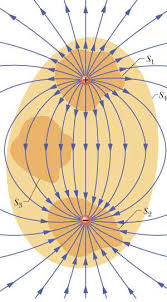
\includegraphics[height=5cm]{img/cariche opposte.jpg}
    	\caption{Due cariche di intensità uguale, ma di segno opposto}
\end{figure}
\begin{itemize}
\item $S_1$: $\vec{E}$ uscente in tutti i punti. $\Phi$ positivo, $q_{int}$ negativa
\item $S_2$: $\vec{E}$ entrante in tutti i punti. $\Phi$ negativa, $q_{int}$ negativa
\item $S_3$ Non racchiude nessuna carica. Ogni linea di campo che entra, esce, quindi $\Phi = 0$
  \item $S_4$ $q_{int}$ = $Q-Q=0$, quindi $\Phi = 0$
\end{itemize}

\section{La legge di Gauss e di Coulomb}
Racchiudiamo una \textbf{carica puntiforme} in una superficie sferica di raggio $r$.
Per simmetria, il campo elettronico ha il medesimo modulo $E$ su \textbf{tutti i punti della sfera}.\\
Applichiamo Gauss:
\begin{eqnarray*}
  \xi_0\oint \vec{E}*d\vec{A}=q_{int}\\
  \xi_0 E(4\pi r^2) = q\\
  E=\frac{q}{4\pi\xi_0r^2}
\end{eqnarray*}
Cioè, la legge di coulomb!
\subsection{Problema svolto}
Guscio sferica di raggio $R=10cm$ - dotato di carica uniforme $Q=-16e$ - Al centro carca puntiforme $q=5e$. Calcolare il campo $\vec{E}$
\begin{itemize}
\item nel punto $P_1$ a $r_1=6cm$
\item nel punto $P_2$ a $r_2=12cm$
\end{itemize}
\begin{eqnarray*}
  \xi_0 E_1(4\pi r_1^2)=q\to E=\frac{q}{4\pi \xi_0 r^2_1}=\frac{4e}{4\pi \xi_0 (0,06m)^2}=2,0*10^{-6}\frac{N}{C} \text{ verso l'esterno}\\
  \xi_0 E_2 (4\pi r^2_2)=q+Q\to \frac{q+Q}{4\pi \xi_0 r^2_2}=\frac{4e}{4\pi \xi_0 (0,12m)^2}=1,1 *10^{-6}\frac{N}{C} \text{ verso l'interno}
\end{eqnarray*}
\section{Un conduttore carico isolato}
Il campo elettrico all'\textit{interno} di un conduttore in equilibrio elettrostatico è \textit{nullo}
\begin{center}
	se no, si spostano le cariche
\end{center}
Scegliamo una superficie gaussiana appena sotto la superficie,


\end{document}
